% Não é necessário alterar nada nesta primeira parte, esta primeira parte consiste na parte de configuração da linguagem e da formatação mais bruta do clipping %

%%%%%%%%%%%%%%%%%%%%%%%%%%%%%%%%%%%%%%%%%%%%%%%%%%%%%%%%%%%%%%%%%
%% Este é um documento que servirá de modelo para os Clippings %%
%%  de Notícias produzidos pela Sala de Situação de Saúde      %%
%% da Faculdade de Saúde - UnB                                 %%
%%%%%%%%%%%%%%%%%%%%%%%%%%%%%%%%%%%%%%%%%%%%%%%%%%%%%%%%%%%%%%%%%




% INÍCIO DA PRIMEIRA PARTE - NÃO ALTERAR NADA %





\documentclass{article}
\usepackage[utf8]{inputenc}
\usepackage{multicol}
\usepackage{caption}
\usepackage{float}
\setlength{\columnsep}{0.5cm}
\usepackage{ragged2e} %Para usar o comando que justifica o texto
\usepackage{graphicx}
\usepackage{wrapfig}
\usepackage{eso-pic}
\usepackage{xcolor} 
\usepackage[hidelinks]{hyperref}
\PassOptionsToPackage{hyphens}{url}
\usepackage[hyphens]{url}
\expandafter\def\expandafter\UrlBreaks\expandafter{\UrlBreaks
  \do\a\do\b\do\c\do\d\do\e\do\f\do\g\do\h\do\i\do\j
  \do\k\do\l\do\m\do\n\do\o\do\p\do\q\do\r\do\s\do\t
  \do\u\do\v\do\w\do\x\do\y\do\z\do\A\do\B\do\C\do\D
  \do\E\do\F\do\G\do\H\do\I\do\J\do\K\do\L\do\M\do\N
  \do\O\do\P\do\Q\do\R\do\S\do\T\do\U\do\V\do\W\do\X
  \do\Y\do\Z} %%% Comando implementado para a quebra de linha nas urls
\hypersetup{
   colorlinks,
   %linkcolor={red!50!black},
   %citecolor={blue!50!black},
   urlcolor={blue!80!black}
}
\usepackage[a4paper, total={8in,6in}]{geometry}
%\usepackage[top=6cm]{geometry}
\usepackage{ifthen}
\usepackage{lipsum}
\pagestyle{empty}%oculta numeracao das paginas 
\newcommand{\cfbox}[2]{%comando de inserção de blocos%
    \colorlet{currentcolor}{.}%
    {\color{#1}%
    \fbox{\color{currentcolor}#2}}%
}

\usepackage{scrextend}
\usepackage{moresize}
\usepackage{fontspec}
\setmainfont[BoldItalicFont=Myriad_Bold_Italic.ttf, BoldFont=MyriadPro-Bold.otf, ItalicFont=MyriadPro-It.otf]{MyriadPro-Regular.otf}

\newfontfamily{\calibrifont}[BoldItalicFont=CalibriBoldItalic.ttf, BoldFont=CalibriBold.ttf, ItalicFont=CalibriItalic.ttf]{Calibri.ttf}
\DeclareTextFontCommand{\calibri}{\calibrifont}
%\fontspec

\date{}

\newcommand\addtopico[2]{
\hspace*{-1in}
\begin{picture}(0,30)
\put(45,0){\includegraphics[width=\paperwidth,height=1cm]{#1.png}}
\put(45,-15){\includegraphics[width=\paperwidth]{#2.png}}
\end{picture}
\\
}

\newcommand\addseccao[1]{
\hspace*{-1in}
\begin{picture}(0,15)
\put(45,0){\includegraphics{#1.png}}
\end{picture}
}

\newcommand\addbox[8]{ %comando que adiciona os blocos, recebe 6 parametros%
\begin{figure}[H]
\cfbox{blue}{
\begin{minipage}{\dimexpr \textwidth-2\fboxsep-2\fboxrule}
\abovecaptionskip=0pt
\caption*{#1}
\sbox0{\includegraphics[scale=#2]{#3.png}}% imagem fixada na coluna esquerda do texto
\hangafter \numexpr -\ht0/\baselineskip\relax% adiciona duas bordas no rodapé do bloco
\hangindent \dimexpr \wd0 + 1em\relax% adiciona uma margem de 1em em relação a imagem
\vbox{\raisebox{-\height}[0pt][15pt]{\box0}}\vspace{-1ex}% intersecciona a imagem com texto
#4
\begin{figure}[H]
\sbox0{\includegraphics[width=.#5\textwidth]{#6}}% get height and width
\hangafter \numexpr -\ht0/\baselineskip -2\relax% adds two blank lines at bottom
\hangindent \dimexpr \wd0 + 25em\relax% adds 1em margin on right
\vbox{\raisebox{-\height}[0pt][0pt]{\hspace*{200pt}\box0}}\vspace{-1ex}% overlap image
#7 \\
\footnotesize\url{#8}
\vskip 0.8cm
\end{figure}
\end{minipage}
}
\end{figure}
}

\newcommand\addboxcolorido[9]{ %comando que adiciona os blocos, recebe 9 parametros sendo um com a cor%
\begin{figure}[H]
\cfbox{blue}{
\colorbox{#9}{\begin{minipage}{\dimexpr \textwidth-2\fboxsep-2\fboxrule}
\abovecaptionskip=0pt
\caption*{#1}
\sbox0{\includegraphics[scale=#2]{#3.png}}% imagem fixada na coluna esquerda do texto
\hangafter \numexpr -\ht0/\baselineskip\relax% adiciona duas bordas no rodapé do bloco
\hangindent \dimexpr \wd0 + 1em\relax% adiciona uma margem de 1em em relação a imagem
\vbox{\raisebox{-\height}[0pt][15pt]{\box0}}\vspace{-1ex}% intersecciona a imagem com texto
#4
\begin{figure}[H]
\sbox0{\includegraphics[width=.#5\textwidth]{#6}}% get height and width
\hangafter \numexpr -\ht0/\baselineskip -2\relax% adds two blank lines at bottom
\hangindent \dimexpr \wd0 + 25em\relax% adds 1em margin on right
\vbox{\raisebox{-\height}[0pt][0pt]{\hspace*{200pt}\box0}}\vspace{-1ex}% overlap image
#7 \\
\footnotesize\url{#8}
\vskip 0.8cm
\end{figure}
\end{minipage}
}
}
\end{figure}
}


% Grupos de tamanho de letra: tiny, scriptsize, footnotesize, small, normalsize, large, Large, huge, Huge. 




% FIM DA PRIMEIRA PARTE - NÃO ALTERAR NADA DA PRIMEIRA PARTE%




\title{Modelo Clipping de Notícias}

\begin{document}
\pagestyle{empty}
\thispagestyle{empty}%oculta numeracao da primeira pagina




%Colocando plando de fundo que possui o cabeçalho do clipping somente na primeira página 
\AddToShipoutPictureBG{\ifthenelse{\value{page}>1}{}{
\includegraphics[width=\paperwidth,height=\paperheight]{fundo_primeira_pag_clipping.pdf}}}


%Colocando plano de fundo nas demais páginas
\AddToShipoutPictureBG{\ifthenelse{\value{page}<2}{}{
\includegraphics[width=\paperwidth,height=\paperheight]{fundo.pdf}}}

\addtopico{BRASIL}{ZIKA} % Esta linha é utilizada para adicionar um novo topico e uma subseccao desse topico, apenas deixe os dois nomes das imagens referentes as imagens do topico que esteja tentando colocar(imagem precisa estar em png), ou seja, você pode colocar Brasil na primeira parte pois indica qual local e pode colocar ZIKA na segunda parte pois indica qual assunto necessário%

%\addbox{ % adiciona um bloco azul na página%
%\centering\large\textbf{Após resultado promissor em %teste, pesquisa deve usar zika vírus contra tumor em %pacientes %título do bloco%
%}}{
%img_noticia_1 %nome da imagem do bloco(.png)%
%}{
%\large %conteúdo do bloco azul%
%Um estudo de pesquisadores da USP (Universidade de %São Paulo), publicado na quinta-feira (26/04) na %revista Cancer Research, conseguiu reduzir o tumor %agressivo do sistema nervoso central em camundongo %com a aplicação do vírus Zika.
%\vskip 0mm
%}{
%3 %tamanho da imagem do bloco%
%}
%{
%logo_not_1 %imagem da logo da noticia(.png)%
%}{
%\calibri{\small{06/05/2018}} %data%
%}{
%https://www.urdupoint.com/en/health/first-dengue-%fever-case-confirmed-in-manshera-336798.html
%link que direciona a página a notícia%
%}
%recomendável padronizar o tamanho das imagens
    

%\addboxcolorido{ comenta nessa funçao 
%\centering\large\textbf{Após resultado promissor em teste, pesquisa deve usar zika vírus contra tumor em pacientes}
%Esta parte define o título da notícia contida no quadrado, para alterar basta trocar a frase que esta na cor preta pela frase desejada 

%}{0.41}{img_noticia_1}{ 
%\large %Está linha é utilizada para aumentar a fonte pois a fonte padrão do latex é menor, não é necessário alterar essa parte, a menos que seja necessário alterar tamanho da fonte. Neste caso, \large pode ser alterado para uma dessas opções da menor para maior: \tiny, \scriptsize, \footnotesize, \small, \normalsize, \arge, \Large, \huge, \Huge .

%Um estudo de pesquisadores da USP (Universidade de São Paulo), publicado na quinta-feira (26/04) na revista Cancer Research, conseguiu reduzir o tumor agressivo do sistema nervoso central em camundongo com a aplicação do vírus Zika.

% Esta parte é utilizada para colocar o texto do primeiro tópico, para alterar basta alterar o que está escrito na cor preta dentro das chaves

% Além da confirmação de novos casos, a variação no número de casos e óbitos entre as publicações se deve em parte à constante revisão e reclassificação dos casos à luz de novos dados que são semanalmente incorporadas à base, à medida que as investigações epidemiológicas dos casos notificados reúnem informações essenciais que trazem implicações à avaliação crítica desses eventos. Assim, pode haver redução no número de casos confirmados quando os casos revisados/reclassificados superarem os casos novos.
% \vskip 0mm
% }{18}{logo_not_2}{\calibri{\small{06/05/2018}}}{https://bhaz.com.br/2018/05/06/surto-doenca-pe-mao/}  % esta linha serve para alterar a data, basta trocar a data que está dentro das chaves%
%esta linha serva para alterar o endereço da notícia, basta trocar o endereço da notícia que esta dentro das chaves

%\cfbox{blue}{\begin{minipage}{55em} %insere um bloco de cor azul na pagina, ou seja, nesta parte é escrito qual cor(em inglês) será o quadrado em volta da notícia (a borda do quadrado), para alterar a cor é apenas necessário trocar "blue" pela cor desejada escrita em inglês% 



%\vskip 0mm
%}{3}{
%logo_not_1
%}{\calibri{\small{06/05/2018}}}
%{https://www.urdupoint.com/en/health/first-dengue-fever-case-confirmed-in-manshera-336798.html}

%\addbox{ comenta nessa funçao 
%\centering\large\textbf{Após resultado promissor em teste, pesquisa deve usar zika vírus contra tumor em pacientes}
%Esta parte define o título da notícia contida no quadrado, para alterar basta trocar a frase que esta na cor preta pela frase desejada 

%}{0.41}{img_noticia_1}{ 
%\large %Está linha é utilizada para aumentar a fonte pois a fonte padrão do latex é menor, não é necessário alterar essa parte, a menos que seja necessário alterar tamanho da fonte. Neste caso, \large pode ser alterado para uma dessas opções da menor para maior: \tiny, \scriptsize, \footnotesize, \small, \normalsize, \arge, \Large, \huge, \Huge .

%Um estudo de pesquisadores da USP (Universidade de São Paulo), publicado na quinta-feira (26/04) na revista Cancer Research, conseguiu reduzir o tumor agressivo do sistema nervoso central em camundongo com a aplicação do vírus Zika.

% Esta parte é utilizada para colocar o texto do primeiro tópico, para alterar basta alterar o que está escrito na cor preta dentro das chaves

% Além da confirmação de novos casos, a variação no número de casos e óbitos entre as publicações se deve em parte à constante revisão e reclassificação dos casos à luz de novos dados que são semanalmente incorporadas à base, à medida que as investigações epidemiológicas dos casos notificados reúnem informações essenciais que trazem implicações à avaliação crítica desses eventos. Assim, pode haver redução no número de casos confirmados quando os casos revisados/reclassificados superarem os casos novos.
% \vskip 0mm
% }{18}{logo_not_2}{\calibri{\small{06/05/2018}}}{https://bhaz.com.br/2018/05/06/surto-doenca-pe-mao/}  % esta linha serve para alterar a data, basta trocar a data que está dentro das chaves%
%esta linha serva para alterar o endereço da notícia, basta trocar o endereço da notícia que esta dentro das chaves

%\cfbox{blue}{\begin{minipage}{55em} %insere um bloco de cor azul na pagina, ou seja, nesta parte é escrito qual cor(em inglês) será o quadrado em volta da notícia (a borda do quadrado), para alterar a cor é apenas necessário trocar "blue" pela cor desejada escrita em inglês% 



%\vskip 0mm
%}{3}{
%logo_not_1
%}{\calibri{\small{06/05/2018}}}
%{https://www.urdupoint.com/en/health/first-dengue-fever-case-confirmed-in-manshera-336798.html}
%{grey} essa seria a cor do bloco, no caso as cores são descritas em inglês, você pode utilizar por exemplo green(verde),red(vermelho),grey(cinza),blue(azul),yellow(amarelo), etc.


\addbox{ 
\centering\large\textbf{Após resultado promissor em teste, pesquisa deve usar zika vírus contra tumor em pacientes}}{0.41}{img_noticia_1}{ 
\large
Um estudo de pesquisadores da USP (Universidade de São Paulo), publicado na quinta-feira (26/04) na revista Cancer Research, conseguiu reduzir o tumor agressivo do sistema nervoso central em camundongo com a aplicação do vírus Zika.
\vskip 5mm
}{3}{logo_not_1}{\calibri{\small{06/05/2018}}}
{https://www.urdupoint.com/en/health/first-dengue-fever-case-confirmed-in-manshera-336798.html} %esta linha serva para alterar o endereço da notícia, basta trocar o endereço da notícia que esta dentro das chaves


\addseccao{OUTRAS_DOENCAS} %adiciona subseccoes%
\vskip -0.4cm
\addbox{ %adiciona um bloco na pagina%
\centering\large\textbf{\textcolor{white}{MINAS GERAIS}}\hspace{\textwidth} %Esta linha serve para colocar qual região é da notícia, para alterar basta trocar o nome da região que esta dentro das chaves


%\addbox{ comenta nessa funçao 
%\centering\large\textbf{Minas registra surtos da síndrome mão-pé-boca este ano}}{0.41}{img_noticia_2}{
%Esta parte define o título da notícia contida no quadrado, para alterar basta trocar a frase que esta na cor preta pela frase desejada
% Este espaço serve para colocar a imagem desejada, a imagem irá aparecer justificado em harmonia com o texto colocado, para alterar a imagem basta inserir a imagem no canto superior esquerdo na aba "project", e assim irá abrir uma nova aba escrito "file", agora é necessário clicar na palavra "files" que está na cor cinza com um ícone de pasta ao lado, quando clicado no ícone "file" irá abrir uma janela com várias opções, aí é necessário selecionar a 9ª opção denominada "computer" que está no subitem uploade... computer, a escolha é de selecionar a imagem do computador e após a escolha é necessário clicar em enviar; após fazer isso é necessário observar qual o nome da imagem, e aí é necessário apenas acrescentar o nome da imagem nas chaves abaixo, conforme exemplo {capa_boletim_epidemiologico.png} é necessário colocar a extensão da imagem (no caso o .png), caso a imagem seja .jpg é necessário alterar o .png para o .jpg %
\large%Está linha é utilizada para aumentar a fonte pois a fonte padrão do latex é menor, não é necessário alterar essa parte, a menos que seja necessário alterar tamanho da fonte. Neste caso, \large pode ser alterado para uma dessas opções da menor para maior: \tiny, \scriptsize, \footnotesize, \small, \normalsize, \arge, \Large, \huge, \Huge .
%     % Esta parte é utilizada para colocar o texto do primeiro tópico, para alterar basta alterar o que está escrito na cor preta dentro das chaves
%Além da confirmação de novos casos, a variação no número de casos e óbitos entre as publicações se deve em parte à constante revisão e reclassificação dos casos à luz de novos dados que são semanalmente incorporadas à base, à medida que as investigações epidemiológicas dos casos notificados reúnem informações essenciais que trazem implicações à avaliação crítica desses eventos. Assim, pode haver redução no número de casos confirmados quando os casos revisados/reclassificados superarem os casos novos.
%\vskip 0mm
%}{18}{logo_not_2}{\calibri{\small{06/05/2018}}}{https://bhaz.com.br/2018/05/06/surto-doenca-pe-mao/}  % esta linha serve para alterar a data, basta trocar a data que está dentro das chaves%
%esta linha serva para alterar o endereço da notícia, basta trocar o endereço da notícia que esta dentro das chaves

%\cfbox{blue}{\begin{minipage}{55em} %insere um bloco de cor azul na pagina, ou seja, nesta parte é escrito qual cor(em inglês) será o quadrado em volta da notícia (a borda do quadrado), para alterar a cor é apenas necessário trocar "blue" pela cor desejada escrita em inglês% 

\centering\large\textbf{Minas registra surtos da síndrome mão-pé-boca este ano}}{0.41}{img_noticia_2}{
Além da confirmação de novos casos, a variação no número de casos e óbitos entre as publicações se deve em parte à constante revisão e reclassificação dos casos à luz de novos dados que são semanalmente incorporadas à base, à medida que as investigações epidemiológicas dos casos notificados reúnem informações essenciais que trazem implicações à avaliação crítica desses eventos. Assim, pode haver redução no número de casos confirmados quando os casos revisados/reclassificados superarem os casos novos.
\vskip 0mm
}{18}{logo_not_2}{\calibri{\small{06/05/2018}}}{https://bhaz.com.br/2018/05/06/surto-doenca-pe-mao/} 

%\cfbox{blue}{\begin{minipage}{55em} %insere um bloco de cor azul na pagina, ou seja, nesta parte é escrito qual cor(em inglês) será o quadrado em volta da notícia (a borda do quadrado), para alterar a cor é apenas necessário trocar "blue" pela cor desejada escrita em inglês% 




%\centering\large\textbf{Após resultado promissor em teste, pesquisa deve usar zika vírus contra tumor em pacientes} % Esta linha é indicada para colocar o título da notícia abordada dentro do quadrado realizado, o título aparecerá centralizado e em negrito, para alterar o título é necessário colocar a frase desejada dentro da chave % 




%\begin{multicols}{2}
%\justifying
%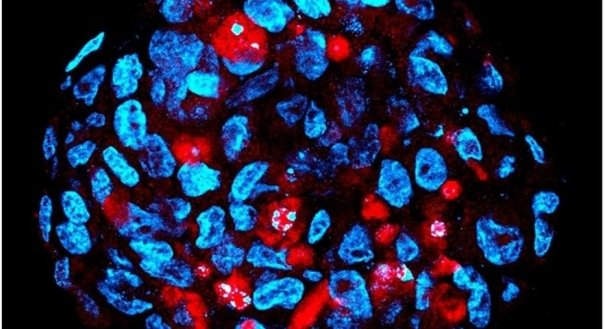
\includegraphics[width=.35\textwidth]{img_noticia_1.png} % Este espaço serve para colocar a imagem necessária dentro do quadrado da notícia, a imagem irá aparecer justificado em harmonia com o texto colocado, para alterar a imagem basta inserir a imagem no canto superior esquerdo na aba "", quando clicado no ícone "" irá abrir uma janela para selecionar a imagem, a escolha é de selecionar a imagem do computador e após a escolha é necessário clicar em enviar; após fazer isso é necessário observar qual o nome da imagem, e aí é necessário apenas acrescentar o nome da imagem nas chaves abaixo, conforme exemplo {img_noticia_1.png} é necessário colocar a extensão da imagem (no caso o .png), caso a imagem seja .jpg é necessário alterar o .png para o .jpg, caso a imagem fique pequena ou grande demais é alterável no número ".35", com a alteração deste número a imagem é alterada de tamanho % 



%\columnbreak
%{\large
%Um estudo de pesquisadores da USP (Universidade de São Paulo), publicado na quinta-feira (26/04) na revista Cancer Research, conseguiu reduzir o tumor agressivo do sistema nervoso central em camundongo com a aplicação do vírus Zika.
%}%%end \large  % Neste espaço é colocado o texto desejado que irá ficar dentro do quadrado da notícia, para alterar este texto é necessário apenas alterar a frase que está na cor preta para a frase desejada %




%{
\includegraphics[width=.3\textwidth]{logo_not_1.png}
%\calibri{\small 06/05/2018}
%\\
%\footnotesize\url{http://cartacampinas.com.br/2018/05/apos-resultado-promissor-em-teste-pesquisa-deve-usar-zika-virus-contra-tumor-em-pacientes/}} % Esta parte insere a imagem desejada abaixo do texto com legenda de data e endereço do site, ara alterar a imagem basta inserir a imagem no canto superior esquerdo na aba "", quando clicado no ícone "" irá abrir uma janela para selecionar a imagem, a escolha é de selecionar a imagem do computador e após a escolha é necessário clicar em enviar; após fazer isso é necessário observar qual o nome da imagem, e aí é necessário apenas acrescentar o nome da imagem nas chaves abaixo, conforme exemplo {logo_not_1.png} é necessário colocar a extensão da imagem (no caso o .png), caso a imagem seja .jpg é necessário alterar o .png para o .jpg, caso a imagem fique pequena ou grande demais é alterável no número ".2", com a alteração deste número a imagem é alterada de tamanho. Para alterar o endereço do site é necessário apenas que altere o http de dentro das chaves % 

%\end{multicols}
%\end{minipage}}
%\cfbox{blue}{\begin{minipage}{55em} %insere um bloco de cor azul na pagina
%\centering\large\textbf{\textcolor{white}{MINAS GERAIS}}

%\centering\large\textbf{Minas registra surtos da síndrome mão-pé-boca este ano}
%\begin{multicols}{2}
%\justifying

%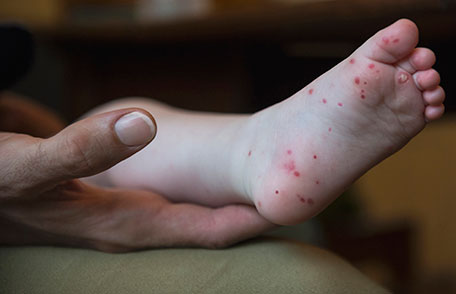
\includegraphics[width=.3\textwidth]{img_noticia_2.png}

%\columnbreak 

% 	Além da confirmação de novos casos, a variação no número de casos e óbitos entre as publicações se deve em parte à constante revisão e reclassificação dos casos à luz de novos dados que são semanalmente incorporadas à base, à medida que as investigações epidemiológicas dos casos notificados reúnem informações essenciais que trazem implicações à avaliação crítica desses eventos. Assim, pode haver redução no número de casos confirmados quando os casos revisados/reclassificados superarem os casos novos.
    
%{
\includegraphics[width=.2\textwidth]{logo_not_2.png}
%  \calibri{\small 06/05/2018}
%\\
%\footnotesize\url{https://bhaz.com.br/2018/05/06/surto-doenca-pe-mao/}}
    
%\end{multicols}
%\end{minipage}}


%\addbox{ comenta nessa funçao 
%\centering\large\textbf{Médico alerta para risco de cegueira em doentes com toxoplasmose}}{1}{img_noticia_3}{ %Esta parte define o título da notícia contida no quadrado, para alterar basta trocar a frase que esta na cor preta pela frase desejada
% Este espaço serve para colocar a imagem desejada, a imagem irá aparecer justificado em harmonia com o texto colocado, para alterar a imagem basta inserir a imagem no canto superior esquerdo na aba "project", e assim irá abrir uma nova aba escrito "file", agora é necessário clicar na palavra "files" que está na cor cinza com um ícone de pasta ao lado, quando clicado no ícone "file" irá abrir uma janela com várias opções, aí é necessário selecionar a 9ª opção denominada "computer" que está no subitem uploade... computer, a escolha é de selecionar a imagem do computador e após a escolha é necessário clicar em enviar; após fazer isso é necessário observar qual o nome da imagem, e aí é necessário apenas acrescentar o nome da imagem nas chaves abaixo, conforme exemplo {capa_boletim_epidemiologico.png} é necessário colocar a extensão da imagem (no caso o .png), caso a imagem seja .jpg é necessário alterar o .png para o .jpg %
\large%Está linha é utilizada para aumentar a fonte pois a fonte padrão do latex é menor, não é necessário alterar essa parte, a menos que seja necessário alterar tamanho da fonte. Neste caso, \large pode ser alterado para uma dessas opções da menor para maior: \tiny, \scriptsize, \footnotesize, \small, \normalsize, \arge, \Large, \huge, \Huge .
     % Esta parte é utilizada para colocar o texto do primeiro tópico, para alterar basta alterar o que está escrito na cor preta dentro das chaves
%Santa Maria já registra 176 pessoas com toxoplasmose. O número foi divulgado nessa sexta-feira (4) pelas secretarias da Saúde do município e do Estado. Ainda há 219 casos em investigação para verificar se são ou não da doença. Pelo menos 681 notificações suspeitas chegaram até agora aos serviços de saúde desde que o surto foi confirmado em abril.
%\vskip 0mm
%}{18}{logo_not_3}{\calibri{\small{06/05/2018}}}{http://jcrs.uol.com.br/_conteudo/2018/04/geral/623937-medico-alerta-para-risco-de-cegueira-em-doentes-com-toxoplasmose.html} % esta linha serve para alterar a data, basta trocar a data que está dentro das chaves%
%esta linha serva para alterar o endereço da notícia, basta trocar o endereço da notícia que esta dentro das chaves

\addbox{ 
\centering\large\textbf{\textcolor{white}{RIO GRANDE DO SUL}}\hspace{\textwidth} 
\centering\large\textbf{Médico alerta para risco de cegueira em doentes com toxoplasmose}}{1}{img_noticia_3}{ 
Santa Maria já registra 176 pessoas com toxoplasmose. O número foi divulgado nessa sexta-feira (4) pelas secretarias da Saúde do município e do Estado. Ainda há 219 casos em investigação para verificar se são ou não da doença. Pelo menos 681 notificações suspeitas chegaram até agora aos serviços de saúde desde que o surto foi confirmado em abril.
\vskip 0mm
}{18}{logo_not_3}{\calibri{\small{06/05/2018}}}{http://jcrs.uol.com.br/_conteudo/2018/04/geral/623937-medico-alerta-para-risco-de-cegueira-em-doentes-com-toxoplasmose.html} 

%\par\cfbox{blue}{\begin{minipage}{55em} %insere um %bloco de cor azul na pagina
%\centering\large\textbf{\textcolor{white}{RIO GRANDE DO SUL}}

%\centering\large\textbf{Médico alerta para risco de cegueira em doentes com toxoplasmose}

%\begin{multicols}{2}
%\justifying
%\includegraphics[width=.3\textwidth]%{img_noticia_3.png}

%\columnbreak

%Santa Maria já registra 176 pessoas com toxoplasmose. O número foi divulgado nessa sexta-feira (4) pelas secretarias da Saúde do município e do Estado. Ainda há 219 casos em investigação para verificar se são ou não da doença. Pelo menos 681 notificações suspeitas chegaram até agora aos serviços de saúde desde que o surto foi confirmado em abril.

%{
\includegraphics[width=.3\textwidth]{logo_not_3.png}
%  \calibri{\small 05/05/2018}
%\\
%\footnotesize\url{http://jcrs.uol.com.br/_conteudo/2018/04/geral/623937-medico-alerta-para-risco-de-cegueira-em-doentes-com-toxoplasmose.html}}

%\end{multicols}
%\end{minipage}}

%\par
%\addbox{ comenta nessa funçao 
%\addbox{ %adiciona um bloco na pagina%
%\centering\large\textbf{\textcolor{white}{PIAUÍ}}\hspace{\textwidth}  %Esta linha serve para colocar qual região é da notícia, para alterar basta trocar o nome da região que esta dentro das chaves
%\centering\large\textbf{Fundação Municipal de Saúde confirma a primeira morte por H1N1 em Teresina}}{1}{img_noticia_4}{ %Esta parte define o título da notícia contida no quadrado, para alterar basta trocar a frase que esta na cor preta pela frase desejada
% Este espaço serve para colocar a imagem desejada, a imagem irá aparecer justificado em harmonia com o texto colocado, para alterar a imagem basta inserir a imagem no canto superior esquerdo na aba "project", e assim irá abrir uma nova aba escrito "file", agora é necessário clicar na palavra "files" que está na cor cinza com um ícone de pasta ao lado, quando clicado no ícone "file" irá abrir uma janela com várias opções, aí é necessário selecionar a 9ª opção denominada "computer" que está no subitem uploade... computer, a escolha é de selecionar a imagem do computador e após a escolha é necessário clicar em enviar; após fazer isso é necessário observar qual o nome da imagem, e aí é necessário apenas acrescentar o nome da imagem nas chaves abaixo, conforme exemplo {capa_boletim_epidemiologico.png} é necessário colocar a extensão da imagem (no caso o .png), caso a imagem seja .jpg é necessário alterar o .png para o .jpg %
%\large%Está linha é utilizada para aumentar a fonte pois a fonte padrão do latex é menor, não é necessário alterar essa parte, a menos que seja necessário alterar tamanho da fonte. Neste caso, \large pode ser alterado para uma dessas opções da menor para maior: \tiny, \scriptsize, \footnotesize, \small, \normalsize, \arge, \Large, \huge, \Huge .
 % Esta parte é utilizada para colocar o texto do primeiro tópico, para alterar basta alterar o que está escrito na cor preta dentro das chaves
%A Fundação Municipal de Saúde de Teresina confirmou neste domingo (6) a primeira morte no Teresina em decorrência de uma infecção pelo vírus da H1N1, conhecida como Gripe A. A vítima trabalhava como motorista e não teve seu nome divulgado.
%\vskip 0mm
%}{18}{logo_not_4}{\calibri{\small{06/05/2018}}}{https://g1.globo.com/pi/piaui/noticia/fundacao-municipal-de-saude-confirma-a-primeira-morte-por-h1n1-em-teresina.ghtml} % esta linha serve para alterar a data, basta trocar a data que está dentro das chaves%
%esta linha serva para alterar o endereço da notícia, basta trocar o endereço da notícia que esta dentro das chaves


\addbox{ 
\centering\large\textbf{\textcolor{white}{PIAUÍ}}\hspace{\textwidth}
\centering\large\textbf{Fundação Municipal de Saúde confirma a primeira morte por H1N1 em Teresina}}{1}{img_noticia_4}{
A Fundação Municipal de Saúde de Teresina confirmou neste domingo (6) a primeira morte no Teresina em decorrência de uma infecção pelo vírus da H1N1, conhecida como Gripe A. A vítima trabalhava como motorista e não teve seu nome divulgado.
\vskip 8mm
}{18}{logo_not_4}{\calibri{\small{06/05/2018}}}{https://g1.globo.com/pi/piaui/noticia/fundacao-municipal-de-saude-confirma-a-primeira-morte-por-h1n1-em-teresina.ghtml}

%\cfbox{blue}{\begin{minipage}{55em} %insere um bloco de cor azul na pagina
%\centering\large\textbf{\textcolor{white}{PIAUÍ}}

%\centering\large\textbf{Fundação Municipal de Saúde confirma a primeira morte por H1N1 em Teresina}

%\begin{multicols}{2}
%\justifying
%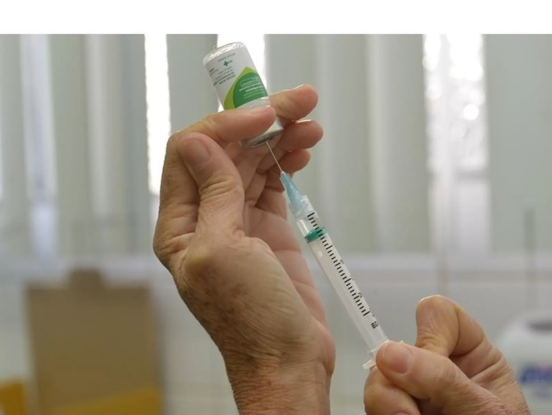
\includegraphics[width=.3\textwidth]{img_noticia_4.png}

%\columnbreak

% 	A Fundação Municipal de Saúde de Teresina confirmou neste domingo (6) a primeira morte no Teresina em decorrência de uma infecção pelo vírus da H1N1, conhecida como Gripe A. A vítima trabalhava como motorista e não teve seu nome divulgado.

%{
\includegraphics[width=.1\textwidth]{logo_not_4.png}
%  \calibri{\small 06/05/2018}
%\\
%\footnotesize\url{https://g1.globo.com/pi/piaui/noticia/fundacao-municipal-de-saude-confirma-a-primeira-morte-por-h1n1-em-teresina.ghtml}}

%\end{multicols}
%\end{minipage}}

\newpage
\addtopico{AMERICA_DO_NORTE}{OUTRAS_DOENCAS} %Serve para alterar o título principal e o subtítulo, para alterar basta colocar a frase desejada dentro das chaves
\vskip 2mm

%\addbox{ comenta nessa funçao 
%\addbox{ %adiciona um bloco na pagina%
%\centering\large\textbf{\textcolor{white}{ESTADOS UNIDOS}}\hspace{\textwidth}  %Esta linha serve para colocar qual região é da notícia, para alterar basta trocar o nome da região que esta dentro das chaves
%\centering\large\textbf{Pesquisadores revelam genes essenciais do parasita da malária}}{0.41}{img_noticia_5}{ %Esta parte define o título da notícia contida no quadrado, para alterar basta trocar a frase que esta na cor preta pela frase desejada
% Este espaço serve para colocar a imagem desejada, a imagem irá aparecer justificado em harmonia com o texto colocado, para alterar a imagem basta inserir a imagem no canto superior esquerdo na aba "project", e assim irá abrir uma nova aba escrito "file", agora é necessário clicar na palavra "files" que está na cor cinza com um ícone de pasta ao lado, quando clicado no ícone "file" irá abrir uma janela com várias opções, aí é necessário selecionar a 9ª opção denominada "computer" que está no subitem uploade... computer, a escolha é de selecionar a imagem do computador e após a escolha é necessário clicar em enviar; após fazer isso é necessário observar qual o nome da imagem, e aí é necessário apenas acrescentar o nome da imagem nas chaves abaixo, conforme exemplo {capa_boletim_epidemiologico.png} é necessário colocar a extensão da imagem (no caso o .png), caso a imagem seja .jpg é necessário alterar o .png para o .jpg %
%\large%Está linha é utilizada para aumentar a fonte pois a fonte padrão do latex é menor, não é necessário alterar essa parte, a menos que seja necessário alterar tamanho da fonte. Neste caso, \large pode ser alterado para uma dessas opções da menor para maior: \tiny, \scriptsize, \footnotesize, \small, \normalsize, \arge, \Large, \huge, \Huge .
     % Esta parte é utilizada para colocar o texto do primeiro tópico, para alterar basta alterar o que está escrito na cor preta dentro das chaves
%Pesquisadores exploraram um capricho na constituição genética do mortal parasita da malária, \textit{Plasmodium falciparum}, para criar 38.000 linhagens mutantes e então determinar quais dos genes do organismo são essenciais para seu crescimento e sobrevivência. O P. \textit{falciparum} é responsável por cerca de metade de todos os casos de malária e 90\% de todas as mortes por malária. Novas informações sobre o repertório de genes críticos do parasita poderiam ajudar os pesquisadores a priorizar alvos para o desenvolvimento futuro de drogas antimaláricas.
%\vskip 0mm
%}{18}{logo_not_5}{\calibri{\small{07/05/2018}}}{http://www.pharmabiz.com/NewsDetails.aspx?aid=108703&sid=2} % esta linha serve para alterar a data, basta trocar a data que está dentro das chaves%
%esta linha serva para alterar o endereço da notícia, basta trocar o endereço da notícia que esta dentro das chaves

\addbox{ 
\centering\large\textbf{\textcolor{white}{ESTADOS UNIDOS}}\hspace{\textwidth} 
\centering\large\textbf{Pesquisadores revelam genes essenciais do parasita da malária}}{0.41}{img_noticia_5}{ 
Pesquisadores exploraram um capricho na constituição genética do mortal parasita da malária, \textit{Plasmodium falciparum}, para criar 38.000 linhagens mutantes e então determinar quais dos genes do organismo são essenciais para seu crescimento e sobrevivência. O P. \textit{falciparum} é responsável por cerca de metade de todos os casos de malária e 90\% de todas as mortes por malária. Novas informações sobre o repertório de genes críticos do parasita poderiam ajudar os pesquisadores a priorizar alvos para o desenvolvimento futuro de drogas antimaláricas.
\vskip 0mm
}{18}{logo_not_5}{\calibri{\small{07/05/2018}}}{http://www.pharmabiz.com/NewsDetails.aspx?aid=108703&sid=2} 

%\cfbox{blue}{\begin{minipage}{55em} %insere um bloco de cor azul na pagina
%\centering\large\textbf{\textcolor{white}{ESTADOS UNIDOS}}

%\centering\large\textbf{Pesquisadores revelam genes essenciais do parasita da malária}	
%\begin{multicols}{2}
%\justifying
%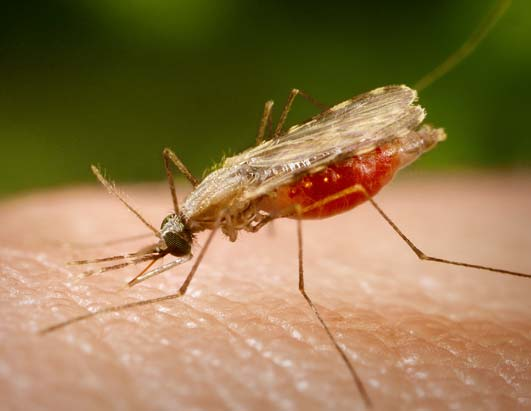
\includegraphics[width=.4\textwidth]{img_noticia_5.png}

%\columnbreak

% 	Pesquisadores exploraram um capricho na constituição genética do mortal parasita da malária, \textit{Plasmodium falciparum}, para criar 38.000 linhagens mutantes e então determinar quais dos genes do organismo são essenciais para seu crescimento e sobrevivência. O P. \textit{falciparum} é responsável por cerca de metade de todos os casos de malária e 90\% de todas as mortes por malária. Novas informações sobre o repertório de genes críticos do parasita poderiam ajudar os pesquisadores a priorizar alvos para o desenvolvimento futuro de drogas antimaláricas.

%{
\includegraphics[width=.3\textwidth]{logo_not_5.png}
% \calibri{\small 07/05/2018}
%\\
%\footnotesize\url{http://www.pharmabiz.com/NewsDetails.aspx?aid=108703&sid=2}}

%\end{multicols}
%\end{minipage}}
\newpage
\addseccao{ZIKA} %esta linha serve para definir qual o assunto principal, para alterar basta trocar o nome desejado dentro das chaves

%\addbox{ comenta nessa funçao 
%\addbox{ %adiciona um bloco na pagina%
%\centering\large\textbf{\textcolor{white}{ESTADOS UNIDOS}}\hspace{\textwidth}  %Esta linha serve para colocar qual região é da notícia, para alterar basta trocar o nome da região que esta dentro das chaves
%\centering\large\textbf{Flórida: Mosquitos que carregam zika podem trazer febre amarela mortal neste ano}}{1}{img_noticia_6}{ %Esta parte define o título da notícia contida no quadrado, para alterar basta trocar a frase que esta na cor preta pela frase desejada
% Este espaço serve para colocar a imagem desejada, a imagem irá aparecer justificado em harmonia com o texto colocado, para alterar a imagem basta inserir a imagem no canto superior esquerdo na aba "project", e assim irá abrir uma nova aba escrito "file", agora é necessário clicar na palavra "files" que está na cor cinza com um ícone de pasta ao lado, quando clicado no ícone "file" irá abrir uma janela com várias opções, aí é necessário selecionar a 9ª opção denominada "computer" que está no subitem uploade... computer, a escolha é de selecionar a imagem do computador e após a escolha é necessário clicar em enviar; após fazer isso é necessário observar qual o nome da imagem, e aí é necessário apenas acrescentar o nome da imagem nas chaves abaixo, conforme exemplo {capa_boletim_epidemiologico.png} é necessário colocar a extensão da imagem (no caso o .png), caso a imagem seja .jpg é necessário alterar o .png para o .jpg %
%\large%Está linha é utilizada para aumentar a fonte pois a fonte padrão do latex é menor, não é necessário alterar essa parte, a menos que seja necessário alterar tamanho da fonte. Neste caso, \large pode ser alterado para uma dessas opções da menor para maior: \tiny, \scriptsize, \footnotesize, \small, \normalsize, \arge, \Large, \huge, \Huge .
     % Esta parte é utilizada para colocar o texto do primeiro tópico, para alterar basta alterar o que está escrito na cor preta dentro das chaves
%O medo de Zika de 2016 pode se transformar em pânico de febre amarela este ano se os moradores do sul da Flórida baixarem a guarda quando se trata de se proteger de mosquitos portadores de doenças.
%\vskip 0mm
%}{18}{logo_not_6}{\calibri{\small{06/05/2018}}}{http://www.pharmabiz.com/NewsDetails.aspx?aid=108703&sid=2} % esta linha serve para alterar a data, basta trocar a data que está dentro das chaves%
%esta linha serva para alterar o endereço da notícia, basta trocar o endereço da notícia que esta dentro das chaves

\addbox{ 
\centering\large\textbf{\textcolor{white}{ESTADOS UNIDOS}}\hspace{\textwidth} 
\centering\large\textbf{Flórida: Mosquitos que carregam zika podem trazer febre amarela mortal neste ano}}{1}{img_noticia_6}{
O medo de Zika de 2016 pode se transformar em pânico de febre amarela este ano se os moradores do sul da Flórida baixarem a guarda quando se trata de se proteger de mosquitos portadores de doenças.
\vskip 0mm
}{18}{logo_not_6}{\calibri{\small{06/05/2018}}}{http://www.pharmabiz.com/NewsDetails.aspx?aid=108703&sid=2} 

\vskip 0.4cm
\addseccao{DENGUE} %esta linha serve para especificar qual o título principal da notícia, para alterar basta alterar o que está dentro das chaves para a frase desejada
\addbox{ %adiciona um bloco na pagina%

%\addbox{ comenta nessa funçao 
%\centering\large\textbf{\textcolor{white}{MUNDO}}\hspace{\textwidth}
%\centering\large\textbf{Dengue pode ser transmitida por via sexual, diz estudo}}{0.85}{img_noticia_7}{%Esta parte define o título da notícia contida no quadrado, para alterar basta trocar a frase que esta na cor preta pela frase desejada
% Este espaço serve para colocar a imagem desejada, a imagem irá aparecer justificado em harmonia com o texto colocado, para alterar a imagem basta inserir a imagem no canto superior esquerdo na aba "project", e assim irá abrir uma nova aba escrito "file", agora é necessário clicar na palavra "files" que está na cor cinza com um ícone de pasta ao lado, quando clicado no ícone "file" irá abrir uma janela com várias opções, aí é necessário selecionar a 9ª opção denominada "computer" que está no subitem uploade... computer, a escolha é de selecionar a imagem do computador e após a escolha é necessário clicar em enviar; após fazer isso é necessário observar qual o nome da imagem, e aí é necessário apenas acrescentar o nome da imagem nas chaves abaixo, conforme exemplo {capa_boletim_epidemiologico.png} é necessário colocar a extensão da imagem (no caso o .png), caso a imagem seja .jpg é necessário alterar o .png para o .jpg %
%\large%Está linha é utilizada para aumentar a fonte pois a fonte padrão do latex é menor, não é necessário alterar essa parte, a menos que seja necessário alterar tamanho da fonte. Neste caso, \large pode ser alterado para uma dessas opções da menor para maior: \tiny, \scriptsize, \footnotesize, \small, \normalsize, \arge, \Large, \huge, \Huge .
 % Esta parte é utilizada para colocar o texto do primeiro tópico, para alterar basta alterar o que está escrito na cor preta dentro das chaves
%Um estudo do Instituto Nacional para Doenças Infecciosas Lazzaro Spallanzani (Inmi), com sede em Roma, na Itália, indicou que o vírus da dengue também pode ser transmitido por via sexual.
%\vskip 0mm
%}{14}{logo_not_7}{\calibri{\small{06/05/2018}}}{https://www.terra.com.br/noticias/ciencia/dengue-pode-ser-transmitida-por-via-sexual-dizestudo,bd5fec87caf12052ee31a17bb668531dvi21n853.html} % esta linha serve para alterar a data, basta trocar a data que está dentro das chaves%
%esta linha serva para alterar o endereço da notícia, basta trocar o endereço da notícia que esta dentro das chaves

\centering\large\textbf{\textcolor{white}{MUNDO}}\hspace{\textwidth}
\centering\large\textbf{Dengue pode ser transmitida por via sexual, diz estudo}}{0.85}{img_noticia_7}{
Um estudo do Instituto Nacional para Doenças Infecciosas Lazzaro Spallanzani (Inmi), com sede em Roma, na Itália, indicou que o vírus da dengue também pode ser transmitido por via sexual.
\vskip 8mm
}{14}{logo_not_7}{\calibri{\small{06/05/2018}}}{https://www.terra.com.br/noticias/ciencia/dengue-pode-ser-transmitida-por-via-sexual-dizestudo,bd5fec87caf12052ee31a17bb668531dvi21n853.html} 

%\cfbox{blue}{\begin{minipage}{55em} %insere um bloco de cor azul na pagina
%\centering\large\textbf{\textcolor{white}{MUNDO}}

%\centering\large\textbf{Dengue pode ser transmitida por via sexual, diz estudo}	
%\begin{multicols}{2}
%\justifying
%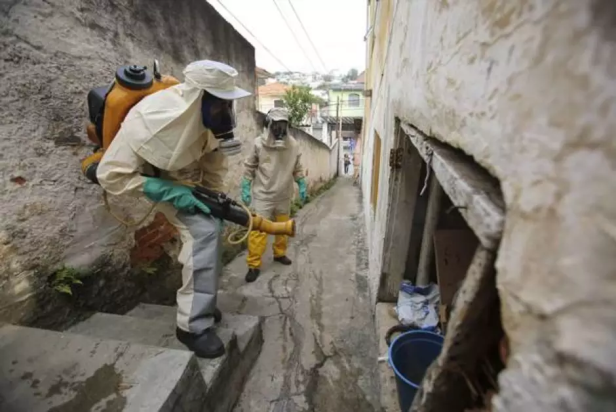
\includegraphics[width=.4\textwidth]{img_noticia_7.png}

%\columnbreak

% 	Um estudo do Instituto Nacional para Doenças Infecciosas Lazzaro Spallanzani (Inmi), com sede em Roma, na Itália, indicou que o vírus da dengue também pode ser transmitido por via sexual.

%{
\includegraphics[width=.1\textwidth]{logo_not_7.png}
%  \calibri{\small 05/05/2018}
%\\
%\footnotesize\url{https://www.terra.com.br/noticias/ciencia/dengue-pode-ser-transmitida-por-via-sexual-dizestudo,bd5fec87caf12052ee31a17bb668531dvi21n853.html}}

%\end{multicols}
%\end{minipage}}
\newpage
\addtopico{AMERICA_LATINA}{OUTRAS_DOENCAS} %esta linha serve para dizer qual o titulo principal e o subtítulo, para alterar basta trocar o que esta dentro das chaves pela frase desejada
\\

%\addbox{ comenta nessa funçao 
%\addbox{ %adiciona um bloco na pagina%
%\centering\large\textbf{\textcolor{white}{MUNDO}}\hspace{\textwidth}  %Esta linha serve para colocar qual região é da notícia, para alterar basta trocar o nome da região que esta dentro das chaves
%\centering\large\textbf{Alerta do Peru: casos de síndrome de Guillain-Barré investigados em Trujillo}}{0.41}{img_noticia_8}{%Esta parte define o título da notícia contida no quadrado, para alterar basta trocar a frase que esta na cor preta pela frase desejada
% Este espaço serve para colocar a imagem desejada, a imagem irá aparecer justificado em harmonia com o texto colocado, para alterar a imagem basta inserir a imagem no canto superior esquerdo na aba "project", e assim irá abrir uma nova aba escrito "file", agora é necessário clicar na palavra "files" que está na cor cinza com um ícone de pasta ao lado, quando clicado no ícone "file" irá abrir uma janela com várias opções, aí é necessário selecionar a 9ª opção denominada "computer" que está no subitem uploade... computer, a escolha é de selecionar a imagem do computador e após a escolha é necessário clicar em enviar; após fazer isso é necessário observar qual o nome da imagem, e aí é necessário apenas acrescentar o nome da imagem nas chaves abaixo, conforme exemplo {capa_boletim_epidemiologico.png} é necessário colocar a extensão da imagem (no caso o .png), caso a imagem seja .jpg é necessário alterar o .png para o .jpg %
%\large%Está linha é utilizada para aumentar a fonte pois a fonte padrão do latex é menor, não é necessário alterar essa parte, a menos que seja necessário alterar tamanho da fonte. Neste caso, \large pode ser alterado para uma dessas opções da menor para maior: \tiny, \scriptsize, \footnotesize, \small, \normalsize, \arge, \Large, \huge, \Huge .
     % Esta parte é utilizada para colocar o texto do primeiro tópico, para alterar basta alterar o que está escrito na cor preta dentro das chaves
%Oito casos de síndrome neurológica aguda compatível com a síndrome de Guillain-Barré foram relatados entre 21 de abril e 1º de maio no Hospital Bethlehem, na cidade de Trujillo, três deles recebem cuidados intensivos com a respiração assistida. Isso levou as autoridades a chamar o público para ir ao centro de saúde se sentirem fraqueza muscular súbita.
%\vskip 0mm
%}{25}{logo_not_8}{\calibri{\small{06/05/2018}}}{http://outbreaknewstoday.com/peru-alert-guillain-barre-syndrome-cases-investigated-trujillo-28439/} % esta linha serve para alterar a data, basta trocar a data que está dentro das chaves%
%esta linha serva para alterar o endereço da notícia, basta trocar o endereço da notícia que esta dentro das chaves

\addbox{ 
\centering\large\textbf{\textcolor{white}{MUNDO}}\hspace{\textwidth} 
\centering\large\textbf{Alerta do Peru: casos de síndrome de Guillain-Barré investigados em Trujillo}}{0.41}{img_noticia_8}{
Oito casos de síndrome neurológica aguda compatível com a síndrome de Guillain-Barré foram relatados entre 21 de abril e 1º de maio no Hospital Bethlehem, na cidade de Trujillo, três deles recebem cuidados intensivos com a respiração assistida. Isso levou as autoridades a chamar o público para ir ao centro de saúde se sentirem fraqueza muscular súbita.
\vskip 0mm
}{25}{logo_not_8}{\calibri{\small{06/05/2018}}}{http://outbreaknewstoday.com/peru-alert-guillain-barre-syndrome-cases-investigated-trujillo-28439/} 

%\cfbox{blue}{\begin{minipage}{55em} %insere um bloco de cor azul na pagina
%\centering\large\textbf{\textcolor{white}{PERU}}

%\centering\large\textbf{Alerta do Peru: casos de síndrome de Guillain-Barré investigados em Trujillo}

%\begin{multicols}{2}

%\justifying
%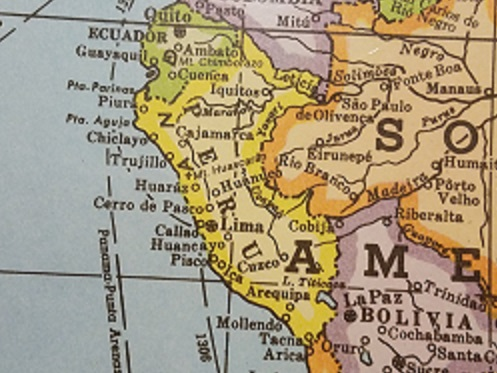
\includegraphics[width=.4\textwidth]{img_noticia_8.png}

%\columnbreak

% 	Oito casos de síndrome neurológica aguda compatível com a síndrome de Guillain-Barré foram relatados entre 21 de abril e 1º de maio no Hospital Bethlehem, na cidade de Trujillo, três deles recebem cuidados intensivos com a respiração assistida. Isso levou as autoridades a chamar o público para ir ao centro de saúde se sentirem fraqueza muscular súbita.

%{
\includegraphics[width=.3\textwidth]{logo_not_8.png}
%  \calibri{\small 07/05/2018}
%\\
%\footnotesize\url{http://outbreaknewstoday.com/peru-alert-guillain-barre-syndrome-cases-investigated-trujillo-28439/}}

%\end{multicols}
%\end{minipage}}

\newpage
\addtopico{ASIA}{DENGUE}  %esta linha serve para dizer qual o titulo principal e o subtítulo, para alterar basta trocar o que esta dentro das chaves pela frase desejada
\\
\\
%\addbox{ comenta nessa funçao 
%\addbox{ %adiciona um bloco na pagina%
%\centering\large\textbf{\textcolor{white}{MUNDO}}\hspace{\textwidth}  %Esta linha serve para colocar qual região é da notícia, para alterar basta trocar o nome da região que esta dentro das chaves
%\centering\large\textbf{Primeiro caso de dengue confirmado em Manshera}}{1}{img_noticia_9}{%Esta parte define o título da notícia contida no quadrado, para alterar basta trocar a frase que esta na cor preta pela frase desejada
% Este espaço serve para colocar a imagem desejada, a imagem irá aparecer justificado em harmonia com o texto colocado, para alterar a imagem basta inserir a imagem no canto superior esquerdo na aba "project", e assim irá abrir uma nova aba escrito "file", agora é necessário clicar na palavra "files" que está na cor cinza com um ícone de pasta ao lado, quando clicado no ícone "file" irá abrir uma janela com várias opções, aí é necessário selecionar a 9ª opção denominada "computer" que está no subitem uploade... computer, a escolha é de selecionar a imagem do computador e após a escolha é necessário clicar em enviar; após fazer isso é necessário observar qual o nome da imagem, e aí é necessário apenas acrescentar o nome da imagem nas chaves abaixo, conforme exemplo {capa_boletim_epidemiologico.png} é necessário colocar a extensão da imagem (no caso o .png), caso a imagem seja .jpg é necessário alterar o .png para o .jpg %
%\large%Está linha é utilizada para aumentar a fonte pois a fonte padrão do latex é menor, não é necessário alterar essa parte, a menos que seja necessário alterar tamanho da fonte. Neste caso, \large pode ser alterado para uma dessas opções da menor para maior: \tiny, \scriptsize, \footnotesize, \small, \normalsize, \arge, \Large, \huge, \Huge .
     % Esta parte é utilizada para colocar o texto do primeiro tópico, para alterar basta alterar o que está escrito na cor preta dentro das chaves
%Primeiro caso de dengue do ano em Manshera foi confirmado no Hospital Abdullah. As autoridades do hospital disseram no sábado que Salman Shah,18 anos de idade, residente de Kohistan , foi internado no hospital poucos dias atrás, onde foi diagnosticado com dengue.
%\vskip 0mm
%}{25}{logo_not_9}{\calibri{\small{06/05/2018}}}{https://www.urdupoint.com/en/health/first-dengue-fever-case-confirmed-in-manshera-336798.html} % esta linha serve para alterar a data, basta trocar a data que está dentro das chaves%
%esta linha serva para alterar o endereço da notícia, basta trocar o endereço da notícia que esta dentro das chaves

\addbox{ 
\centering\large\textbf{\textcolor{white}{MUNDO}}\hspace{\textwidth}  
\centering\large\textbf{Primeiro caso de dengue confirmado em Manshera}}{1}{img_noticia_9}{
Primeiro caso de dengue do ano em Manshera foi confirmado no Hospital Abdullah. As autoridades do hospital disseram no sábado que Salman Shah,18 anos de idade, residente de Kohistan , foi internado no hospital poucos dias atrás, onde foi diagnosticado com dengue.
\vskip 0mm
}{25}{logo_not_9}{\calibri{\small{06/05/2018}}}{https://www.urdupoint.com/en/health/first-dengue-fever-case-confirmed-in-manshera-336798.html} 

%\cfbox{blue}{\begin{minipage}{55em} %insere um bloco de cor azul na pagina
%\centering\textbf{\textcolor{white}{PAQUISTÃO}}

%\centering\normalsize\textbf{Primeiro caso de dengue confirmado em Manshera}

%\begin{multicols}{2}
%\justifying
%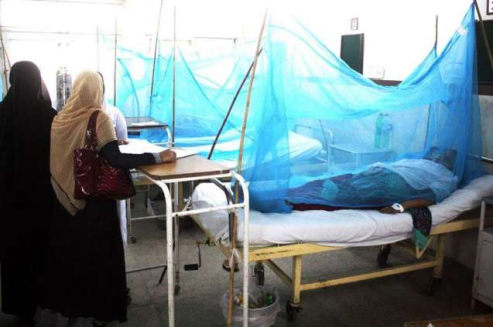
\includegraphics[width=.3\textwidth]{img_noticia_9.png}

%\columnbreak

%Primeiro caso de dengue do ano em Manshera foi confirmado no Hospital Abdullah. As autoridades do hospital disseram no sábado que Salman Shah,18 anos de idade, residente de Kohistan , foi internado no hospital poucos dias atrás, onde foi diagnosticado com dengue.

%{
\includegraphics[width=.3\textwidth]{logo_not_9.png}
%	\calibri{\small 05/05/2018}
%\\
%\footnotesize\url{https://www.urdupoint.com/en/health/first-dengue-fever-case-confirmed-in-manshera-336798.html}}

%\end{multicols}
%\end{minipage}}

\newpage

%\newpage %Próxima página
% referencias do modelo %
\vfill % adiciona as referencias no rodape da pagina%
\centering{

\includegraphics{logo.png} \\
  \normalsize{\bf{\calibrifont Elaboração}}\\
  \calibri{Marina Pissurno}\\
  \normalsize{\bf{\calibrifont Tradução}}\\
  \calibri{Marina Pissurno}\\
  \normalsize{\bf{\calibrifont Equipe Editorial}}\\
  \calibri{Joaquim Bastos\\
  Sala de Situação - Faculdade de Ciências da Saúde (UnB)}\\
  \normalsize{\bf{\calibrifont Revisão}}\\
  \calibri{Patrícia Paiva Pereira, Marcela Lopes Santos}\\
}


\end{document}
